\subsection{Overview}
The architecture of the S2B is a distributed client-server architectural design, structured according to three logic layers:
\begin{itemize}
	\item \textbf{Presentation level P}: manages the user interaction with the system. This layer contains the interfaces able to provide the functions of the application to the users.\\
	To the presentation layer belong the web app, the phone application and the software on the ticket printer and on the QR reader.
	\item \textbf{Business logic or Application layer (A)}: handles the business logic of the application and its functionalities. This layer represent the core of the application logic.
	\item \textbf{Data access layer (D)}: manages information and data, by accessing the database.  
\end{itemize}
Every logic layer can be mapped in an hardware layer.\\
The presentation layer is composed by the smartphone or the computer of the user, the ticket printer outside the stores, the QR reader and the turnstiles.\\
The application layer is composed by the application server.
The data layer is composed by the database server.\\\\\\
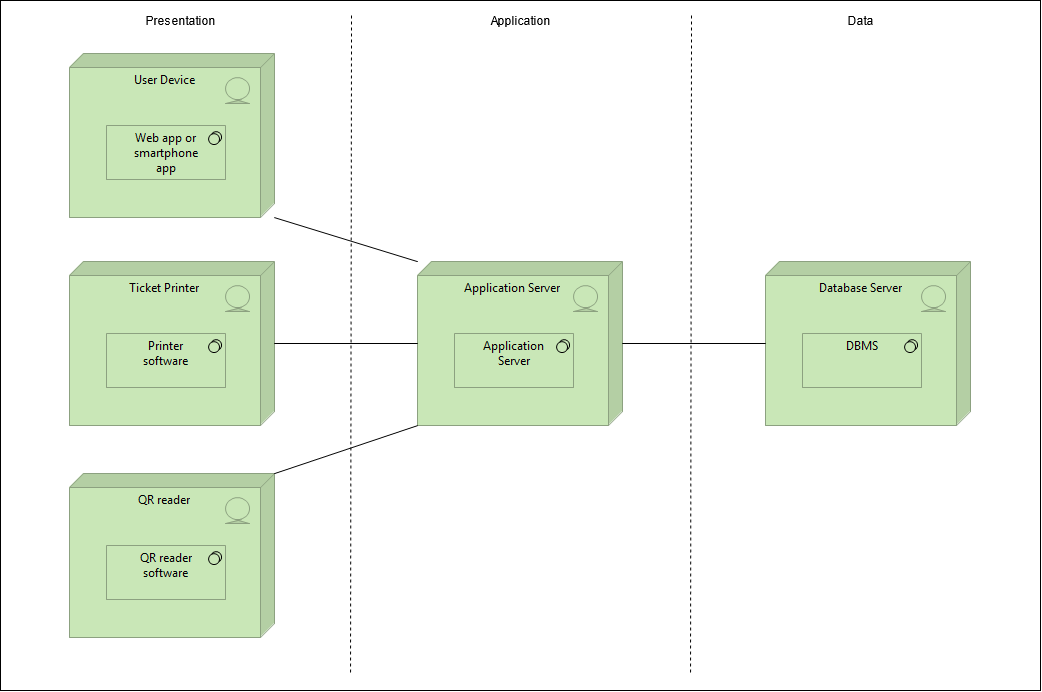
\includegraphics[scale=0.4]{Images/Archimate.png}\\
Customers line up at a store trough the web app or the smartphone application and their requests are sent to the 
\newpage
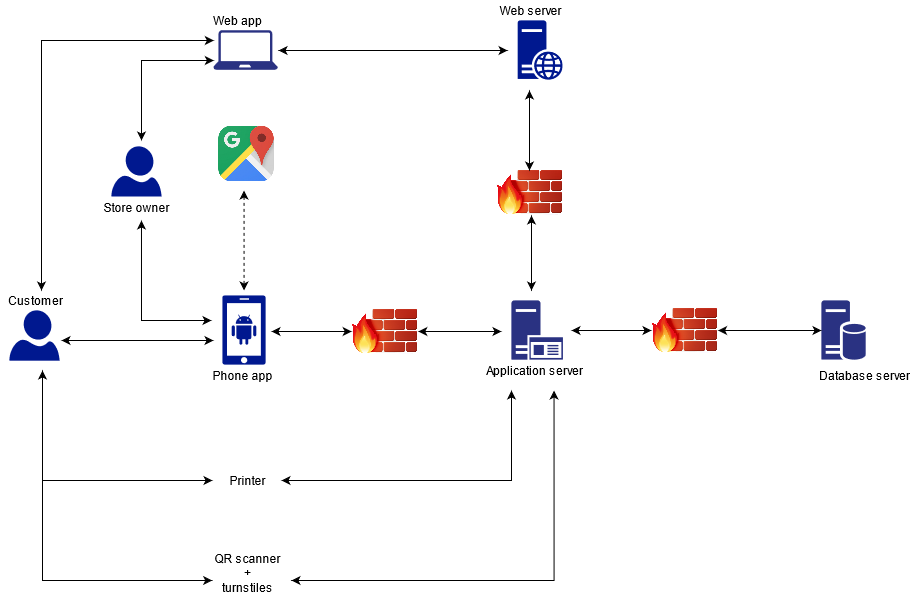
\includegraphics[scale=0.5]{Images/System Architecture.png}\\
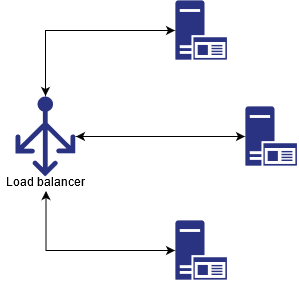
\includegraphics[scale=0.5]{Images/LoadBalancer.png}\\